% thesis.tex
%
% This file is root file for an example thesis written using the
% IIT Guwahati LaTeX Style file.

% The IIT Guwahati LaTex Style is a modified
% version of IIT Bombay LaTex Style created by
% Dr. Amey Karkare (21 June 2007).
%
% Required permissions have been taken from Dr. Karkare in order to
% create the IIT Guwahati LaTex Style using his original work.
% Revision done by: Mandar Kulkarni, EEE Department, IIT Guwahati
% Further revised by Dr. Sonali Chouhan, EEE Department, IIT Guwahati (16/04/2016)

%=====================================================================
% Read: README.txt for more information
%=====================================================================

%=====================================================================
% DOCUMENT STYLE
%=====================================================================
% IITG Thesis format default settings are:
%   12pt, one-sided printing on a4 size paper
\documentclass{iitgthesis}
% For two-sided printing, with Chapter starting on odd-numbered pages,
% use the following line instead:
%%\documentclass[openright,twoside]{iitgthesis}

%=====================================================================
% OPTIONAL PACKAGES
%=====================================================================
% To include optional packages, use the \usepackage command.
% For e.g., The package epsfig is used to bring in the Encapsulated
%    PostScript figures into the document.
%    The package times is used to change the fonts to Times Roman;
%=====================================================================
\usepackage{epsfig}
\usepackage{stackrel}
\usepackage{epsf}
\usepackage{amssymb}
\usepackage{amsthm}
\usepackage{graphicx}
\usepackage{wrapfig}
\usepackage[english]{babel}
\usepackage{mathrsfs}
%\usepackage{fancyhdr}
\usepackage{verbatim}
\usepackage{amsmath,amssymb}

\usepackage{cite}
\usepackage{multirow,tabularx}
\usepackage{ifthen}
% Add these after the document class declaration
\usepackage{times}
\DeclareMathAlphabet{\mathpzc}{OT1}{pzc}{m}{it}

\usepackage{setspace}
\usepackage{amssymb}
%\usepackage{dsfont}
%\usepackage{stmaryrd}
\usepackage{amsmath}
\usepackage{mathrsfs}
\usepackage{array}
%=====================================================================
%  Single counter for theorems and theorem-like environments:
%=====================================================================
\newtheorem{thm}{Theorem}[section]
\newtheorem{theorem}{{\bf Theorem}}
\newtheorem{lemma}{{Lemma}}
\newtheorem{proposition}[theorem]{Proposition}
\newtheorem{corollary}{{\bf Corollary}}
\newtheorem{result}{{\bf Result}}

%=====================================================================
% NEW COMMANDS DEFINED FOR A EASY TO READ CODE
% You are free to add your own set of new commands here
%
\newcommand{\brac}[1]{\left({#1}\right)}
\newcommand{\sbrac}[1]{\left[{#1}\right]}
\newcommand{\cbrac}[1]{\left\{{#1}\right\}}
\newcommand{\expc}[2][]{E_{#1}\left[{#2}\right]}

% End of Preamble, start of document
\graphicspath{ {./} }
%
\begin{document}

\begin{spacing}{1.4}

%=====================================================================
% Include the prelude for Title page, abstract, table of contents, etc
% You need to modify it to contain your details
% prelude.tex
%   - titlepage
%   - dedication (optional)
%   - approval sheet
%   - course certificate
%   - table of contents, list of tables and list of figures
%   - nomenclature
%   - abstract
%============================================================================


\clearpage\pagenumbering{roman}  % This makes the page numbers Roman (i, ii, etc)



% TITLE PAGE
%   - define \title{} \author{} \date{}
\title{VLSI Architectures for Long Short Term Memory Networks}
\author{Author}
\date{November 2018}

%  - Roll number, required for title page, approval sheet, and
%    certificate of course work
\rollnum{150102077) \vspace{0.5}   (Roll No. 150102060}
\author{Krishna Praveen Yalamarthy \hspace{1}   Saurabh Dhall}

%   - The default degree is ``Doctor of Philosophy''
%     (unless the document style msthesis is specified
%      and then the default degree is ``Master of Science'')
%     Degree can be changed using the command \iitbdegree{}
\iitgdegree{Bachelor of Technology}

%   - The default report type is preliminary report.
%      * for a PhD thesis, specify \thesis
\thesis
%      * for a M.Tech./M.Phil./M.Des./M.S. dissertation, specify \dissertation
%\dissertation
%      * for a DIIT/B.Tech./M.Sc.project report, specify \project
%\project
%      * for any other type, use  \reporttype{}
%\reporttype{ReportType}

%   - The default department is ``Unknown Department''
%     The department can be changed using the command \department{}
\department{DEPARTMENT OF ELECTRONICS \& ELECTRICAL ENGINEERING}

%    - Set the guide's name
\setguide{Prof. Rafi Ahmed}

%   - once the above are defined, use \maketitle to generate the titlepage
\maketitle

%--------------------------------------------------------------------%
% APPROVAL SHEET
%   - for final thesis, you need Approval Sheet. So, uncomment the
%     \makeapproval command.
%     it should come after dedication, if dedication is
%     present. Otherwise it is the first page after title page.
%\makeapproval


%--------------------------------------------------------------------%
% COPYRIGHT PAGE
%   - To include a copyright page use \copyrightpage
% \copyrightpage

%--------------------------------------------------------------------%

% ACKNOWLEDGMENTS (optional)
\begin{acknowledgments}
Sample Acknowledgement
\end{acknowledgments}


% ABSTRACT
\begin{abstract}

Long Short Term Memory Networks, which are a modification of the traditional Recurrent Neural Networks, have gained widespread integration into commercial applications to accomplish tasks in the domains of speech recognition, handwriting recognition and are currently deployed in many embedded devices. These networks are computationally expensive and require considerable memory and storage bandwidth which restricts their further use in resource constrained devices. There has been considerable work on optimizing these networks at an algorithmic level, yet there is little to no work being done to reduce the computational complexity on an architectural level using VLSI-DSP techniques. Intially, state-of-art model compression techniques such as Pruning, Quantization, Knowledge distillation are exlpored to decrease the size of the model itself. The next major component of the thesis concentrates on using Distributed Arithmetic to trade computational complexity with ROM lookups. 

\end{abstract}


%--------------------------------------------------------------------%
% CONTENTS, TABLES, FIGURES
\tableofcontents
%\listoftables
\listoffigures

%--------------------------------------------------------------------%
% NOMENCLATURE
%\begin{nomenclature}
%\begin{description}
%\item{\makebox[0.75in][l]{{SN1}}} Sample Nomenclature 1

%\item{\makebox[0.75in][l]{{SN2}}} Sample Nomenclature 2

%\end{description}
%\end{nomenclature}

\cleardoublepage\pagenumbering{arabic} % Make the page numbers Arabic (1, 2, etc)


%=====================================================================
% Include the technical part of the report
\chapter{Introduction}
\label{chap:intro}
\section{VLSI Design Flow}
The development cycle of any digital IC is governed by a few fundmanetal steps or processes that are sequentially followed. The first step begins with designing an algorithm to solve the problem and meet the requirements. Coming up with an algorithm is followed by designing an architecture which can be realized on hardware that is feasible in the desired resource-constrained use case. Different architectures can be proposed for the same algorithm which can be further optimized at the gate level. As shown in the figure \ref{fig:vlsi}, in order to fully exploit the benefit of having an ASIC design, after the gate level modelling, transistor level optimizations are also important. The last stage of the design cycle ends with modifications at the device level.

A small modification at an earlier level in the design flow can lead to a significant change at a later level. A single multiplier that could be eliminated at the architectural level would lead to saving thousands of transistors indicating the significance of higher level optimizations. Since the effects of an optimization are reflected in the following stages, it is essential to fully explore the various possible models or designs.

\begin{figure}[h]
\label{fig:vlsi}
	\caption{VLSI Design Flow}    
    \centering
    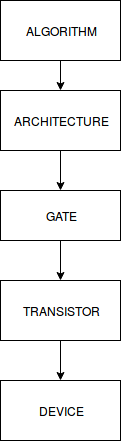
\includegraphics[width=0.1\textwidth]{vlsi_dESIGN}
\end{figure}

\section{Machine Learning}
The field of machine learning is not one that is new. These algorithms have been in existence for a long time although only in recent years they have come into popularity, especially neural networks and deep learning, thanks to the rapid increase in computational power. The GPU has aided in increasing the scale of these models to actually work effectively on real-world tasks. While major strides have been made in improving these algorithms by extensive training and refinement at an algorithmic level, research into architectural changes has been limited. \\
Due to recent advancements in compute power in embedded/mobile device, there is now a possibility of implementing these computationally expensive models on devices with a tighter power, memory and compute constraint than was previously there on non-mobile devices. \\
Indicative of the growing interest in embedded implementations of such networks, in the last couple of years there have been some works on FPGA deployment of LSTMs but none of them seem to leveraging the VLSI digital signal processing techniques for optimization.% [refs to these works] 
VLSI DSP techniques such as systolic arrays, unfolding, distributed arithmetic, CORDIC, pipelining etc., have been in use for the past 30 years for the fields of communication, filters, image processing lend themselves really well for machine learning algorithms as well. Recent work inspired by these techniques optimize Support Vector Machines and Convolutional Neural Networks.%[refs to Rafis papers] 
One branch of neural networks that is explicitly suited for tasks that are applicable in mobile devices are Recurrent Neural Networks. These networks are suited for data that is sequential in nature and have been shown to be effective at tasks such as handwriting recognition and generation, speech and speaker recognition, language modelling, speech synthesis to name a few. \\

\section{Literature Review}
A specialised version of the RNN that is extremely popular for commercial application is the Long Short Term Memory network (LSTM). It is adept at establishing long term dependencies in data . As of 2016, many software giants such as Google, Apple and Microsoft had LSTMs as a fundamental unit in their products. Google incorporated LSTMs for the speech recognition task on the handheld device and also into their smart assistant as well as Google Translate. \\
\\
The typical computational power required by LSTMs is demanding. The challenge of deploying these models is further increased due to the size of the models themselves which needs to be stored locally to fully execute these tasks. 

-original paper
-lstm odyssey
-compression papers
-no proper application of VLSI DSP in this field. can lead to significant improvement to help deploy on devices.

\section{Problem Formulation}
Our goal is to leverage both the best of the available algorithmic optimizations or a combination of those followed by VLSI DSP techniques that are suited to exploit some unique properties of LSTM.
% change to third person
We will first go through the preliminaries that establish the algorithm of Long Short Term Memory Networks. We will then systematically go through the different levels of optimization, from algorithmic to an architectural level, that can be applied to these networks.
        % Chapter 1: Introduction
\chapter{Recurrent Neural Networks}

Any supervised deep learning algorithm consists of primarily two phases i.e., training and inference. Training is where the network is operated on a dataset consisting of input features, like a speech segment, and the associated correct output, as in this case the word it represents. Once the model has been trained it has the capability to predict the output given a completely new input to an extent of accuracy that is determined the training scheme, the model, the dataset and various other parameters. We now elaborate on the model of a recurrent neural network, illustrate its operation and training mechanism and then explain in detail the model of a Long Short Term Memory Network (LSTM).

\section{RNN Structure}
The Recurrent Neural Network consists of a hidden state that is updated on every new input to the network. The updating of the hidden state of the network is influenced by both the previous state of the network and the new input. The output of the network depends on the hidden state of the network. For a single hidden layer the network can be formulated as follows.
Let the hidden state vector be represented by $\mathbf{h}_t\in\mathbb{R}^{m}$ where $m$ is the dimensionality of the hidden state vector at time step $t$. $\mathbf{x}_t\in\mathbb{R}^{n}$ is the input vector and the output vector is $\mathbf{y}_t\in\mathbb{R}^{k}$ at time step $t$.

\begin{equation}
\mathbf{h}_t = f_W(\mathbf{h}_{t-1},\mathbf{x}_t)
\end{equation}
\begin{equation}
\mathbf{h}_t = tanh(\mathbf{W}_{hh}\mathbf{h}_{t-1} + \mathbf{W}_{xh}\mathbf{x}_t)
\end{equation}
\begin{equation}
\mathbf{y}_t = \mathbf{h}_{hy}\mathbf{h}_t
\end{equation}

\begin{figure}[h]
	\caption{Single Layer RNN}    
    \centering
    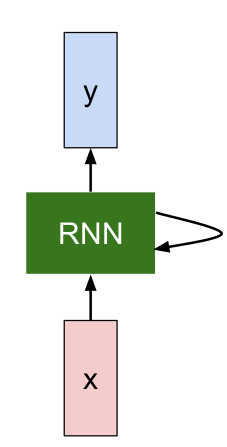
\includegraphics[width=0.1\textwidth]{rnnvanilla}
\end{figure}

The above equations are applied on every new input. The matrices $\mathbf{W}$ represent the connections between the input vector $\mathbf{x}$ and the hidden vector $\mathbf{h}$ as well as the connections between the hidden state and the output vector $\mathbf{y}$. The non-linear function $tanh$ compresses each scalar in the hidden vector to a value between -1 and 1. This non-linearity is crucial to the performance of the network. \\
These connection matrices, more commonly known as weight matrices, are what determine the networks behaviour. The choice of the dimensions of $h$ and the number of hidden layers used determines the capacity of a network to effectively work on the task it is designed for. \\
A good way to visualize the functioning of the network is to observe its behaviour across multiple time steps and and observe the flow of data between the output, the input and within the cell itself. In ~\ref{fig:unroll}, every vertical column of cells represents the same network but at different time instansts.

\begin{figure}[h]
\caption{Unfolded RNN Cell}
\centering
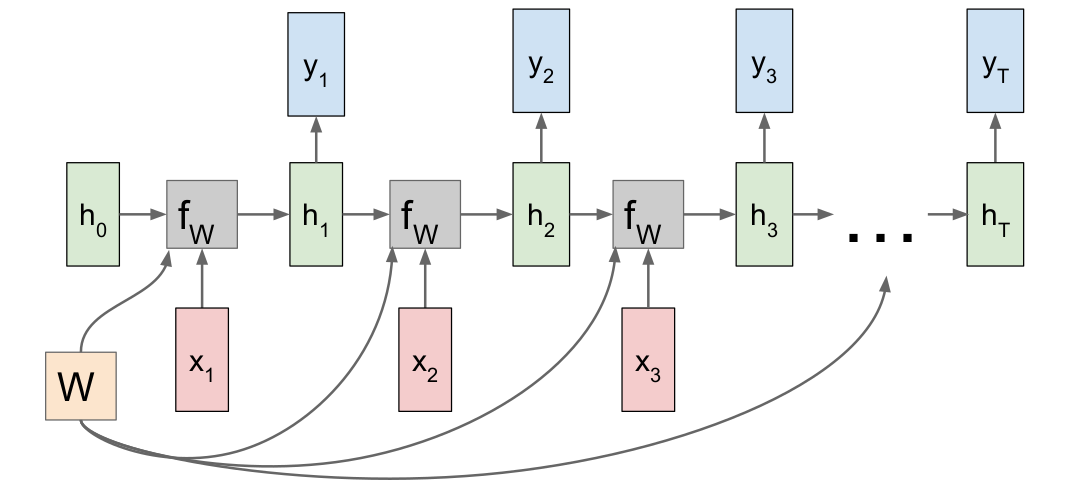
\includegraphics[width=0.8\textwidth]{manyTomany}
\label{fig:unroll}
\end{figure}


A salient point to be noted in recurrent neural networks is that the weight matrices are constant throughout every iteration of the algorithm. This causes some restrictions on what the network is capable of learning:

\begin{enumerate}
    \item The network is poor at learning dependencies between inputs that are separated too far apart as the state of the network tends to slowly forget its past inputs.
    \item During training, the repetition of the matrix causes some terms in the calculation of the training algorithm to explode to infinity or to zero. 
\end{enumerate}
Due to these limitations, a modification of the network known as Long Short Term Memory Networks has been proposed which we will elaborate below.

\section{Long Short Term Memory Networks}
LSTMs were initially introduced by Hochreiter & Schmidhuber in 1997 and through various works was refined into the algorithm used today. An LSTM is a modification of an RNN with additional gates added to it. It consists of three gates that control the flow of information between the input, the hidden state and the output. [ref colahs blog and space]
Let there be:
\begin{enumerate}
    \item Input Connection Weights: $\mathbf{W}_z, \mathbf{W}_s, \mathbf{W}_f, \mathbf{W}_o$ \in $R^{NXM}$ 
    \item Hidden State Weights: $\mathbf{R}_z, \mathbf{R}_s, \mathbf{R}_f, \mathbf{R}_o \in R^{NXN}$
    \item Bias Weights: $\mathbf{b}_z, \mathbf{b}_s, \mathbf{b}_f, \mathbf{b}_o \in R^{N}$
\end{enumerate}
The governing equations of the LSTM update in a time step are as follows:
\begin{equation}
\mathbf{z}^t = \mathbf{W}_z\mathbf{x}^t + \mathbf{R}_z\mathbf{y}^{t-1} + \mathbf{b}_z 
\end{equation}
\begin{equation}
\mathbf{i}^t = \mathbf{W}_i\mathbf{x}^t + \mathbf{R}_i\mathbf{y}^{t-1} + \mathbf{b}_i
\end{equation}
\begin{equation}
\mathbf{i}^t = sigmoid(\mathbf{i}^t)
\end{equation}
\begin{equation}
\mathbf{f}^t = \mathbf{W}_f\mathbf{x}^t + \mathbf{R}_f\mathbf{y}^{t-1} + \mathbf{b}_f
\end{equation}
\begin{equation}
\mathbf{f}^t = sigmoid(\mathbf{f}^t)
\end{equation}
\begin{equation}
\mathbf{c}^t = \mathbf{z}^t\odot\mathbf{i}^t + \mathbf{c}^{t-1}\odot\mathbf{f}^t
\end{equation}
\begin{equation}
\mathbf{o}^t = \mathbf{W}_o\mathbf{x}^t + \mathbf{R}_o\mathbf{y}^{t-1} + \mathbf{b}_o
\end{equation}
\begin{equation}
\mathbf{o}^t = sigmoid(\mathbf{o}^t)
\end{equation}

\begin{equation}
\mathbf{y}^t = tanh(\mathbf{c}^t)\odot\mathbf{o}^t
\end{equation}
$\odot$ represents point-wise multiplication and sigmoid is a logistic function with the following equation 
\[sigmoid(\mathbf{x}) = \frac{1}{1+exp(-\mathbf{x})}\]\\


\begin{figure}[h]
\caption{Graphical representation of an LSTM cell}
\centering
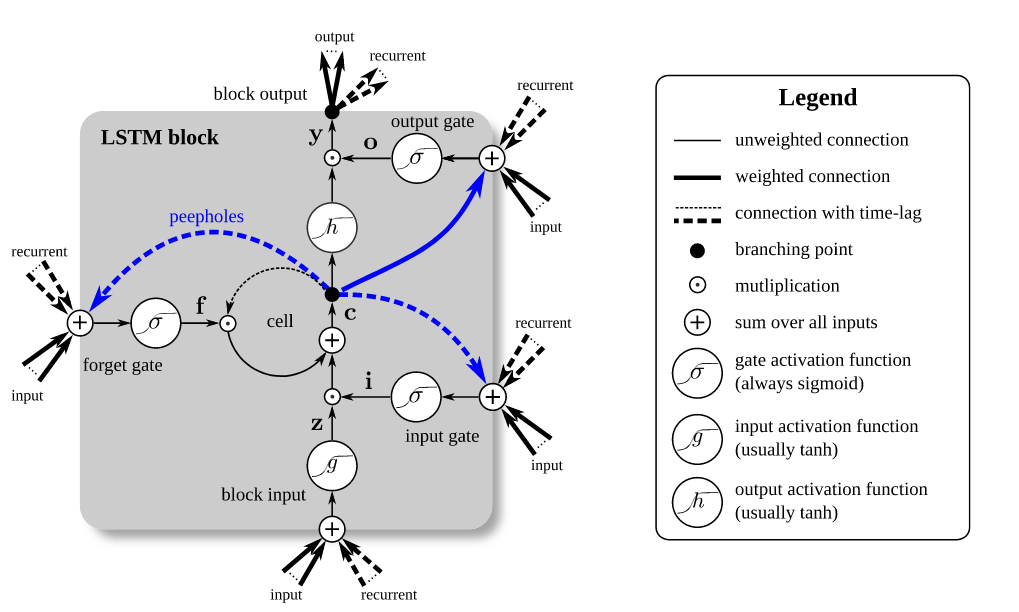
\includegraphics[width=\textwidth]{lstm}
\end{figure}


Each gate serves a purpose: the forget gate controls how much of the previous state is to be retained in the next update, the input gate dictates the influence the new input will have on the state and the output gate controls how much of the output is influence by the hidden state. Due to the addition of these gates, the network has the ability to $remember$ long term dependencies from the input and can solve complex tasks on sequential data.

\subsection{Multi-Layer LSTM}
\begin{figure}[h] 
	\caption{Multi-Layer RNN}    
    \centering
    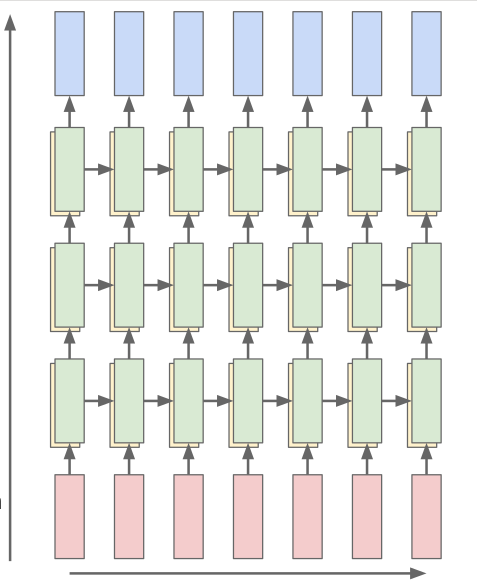
\includegraphics[width=0.25\textwidth]{multi-layer}
\end{figure}
In most state-of-art implementations a single hidden layer isn't used i.e., there isn't just one cell between the input and the output but multiple. This leads to a deep LSTM or a multi-layer LSTM.
\subsection{Google LSTM}


%\section{TIMIT Dataset and Baseline Model}
%In order to compare the results of the various tradeoffs between proposed models and also in order to compare the performance of our final model with others implemented, we need to choose a baseline trained model with optimal performance. The dataset we will be using for this purpose is the TIMIT Acoustic-Phoentic Continuous Speech Corpus. (cite: Garofolo, John S., et al. TIMIT Acoustic-Phonetic Continuous Speech Corpus LDC93S1. Web Download. Philadelphia: Linguistic Data Consortium, 1993.) The dataset contains recordings of 630 speakers covering most of the primary dialects of English, speaking sentences that are phonetically rich. This particular dataset is considered to be a standard for Automatic Speech Recognition Systems and is the dataset of choice for most studies comparing their results with those previously.



         % Chapter 2: Literature survey
\chapter{Network Compression}
The size of deep neural networks has been a major hindrance to their implementation on resource constrained hardware devices. The weight matrix sizes consume significant storage and memory bandwidth. Changes on an algorithmic level have been proposed extensively in the last couple of years with regards to reducing the model sizes of deep neural networks. Reducing the number of parameters, not only allows for faster and less distributed training, but for more power-aware inference which is the aim of our work.\\
Compression of a network, as discussed above, is the reduction of the number of parameters in the model/network. The method of reduction of parameters influences the training method in a unique way ie, the training phase is aware of the compression and must account for the model changes. From recent literature, two broad paradigms have emerged, namely:
\begin{enumerate}
    \item Low Displacement Rank Networks
    \item Pruning and Quantization
    \item Knowledge Diffusion
\end{enumerate}

\section{Low Displacement Rank Networks}

This method of compression takes advantage of the structured nature of certain types of matrices to reduce the number of unique parameters from On2 to On. This not only reduces the storage complexity from On2 to On, it also reduces, due to fast matrix multiplication methods, the computational complexity roughly from On2 to Onlogn or Onlogn2. It uses the fact that any matrix can be compressed to a Low Displacement Rank matrix M which after being computed using the appropriate operation, is decompressed back to the desired result. For deep neural networks, an error bound has been proven for such approximations on the performance of a neural network. \\
Examples of structured matrices are: Circulant, Toeplitz, Henkel, Vandermonde, Cauchy. The predictable structure of these matrices reduces the number of parameters and also eases the indexing process due to its predictability, a lack of which affects the first two methods hence increasing the potential optimization that is possible beforehand when designing an ASIC/FPGA implementation. The other added advantage with respect to the pruning method elaborated below is that there is no iterative training process after introducing the compression as the entire training mechanism is aware of the exact structure of the matrix from the beginning. A recent work uses Circulant matrices as suggested to train the network and achieve a significant speedup on their FPGA implementation of LSTMs.


\section{Pruning and Quantization}
\subsection{Pruning}
In a trained neural network, the weight matrix consists of parameter values that vary drastically in magnitude. Similar to the connections amongst neurons, according to the function that the network is trying to imitate, only certain connections are of computational importance. Hence those connections that have a small magnitude can be removed to increase the sparsity of the network. The state-of-art implementation of such a deep neural network pruning scheme is Deep Compression. We will illustrate the technique suggested and adopt the same to reduce the network size and also explore the different avenues of optimization this creates in the Distributed Arithmetic section.\\
Procedure in training phase: (flow chart insert if possible):
\begin{enumerate}
    \item Train the network at its full capacity.
    \item Prune small magnitude connections by setting a threshold.
    \item Retrain the remaining connections for fine-tuning.
\end{enumerate}

\begin{figure}[h] 
	\caption{A $4X4$ matrix pruned with a threshold magnitude of 0.25}    
    \centering
    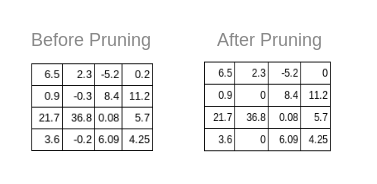
\includegraphics[width=0.25\textwidth]{pruning}
\end{wrapfigure}

\subsection{Quantization}
Further reduction of the model size is possible by quantizing the remaining parameters to K levels. The standard procedure to do this is through K-means clustering. Therefore only logK bits will be required to store the parameters. Literature shows that the two practices of pruning and quantization can be combined together to provide significant drop in the model size. Although the practice of quantization is helpful in reducing the storage bandwidth, it is yet to be used as an way to reduce the implementation of the network. 



             % Chapter 3: System model and formulating the problem statement
\chapter{Distributed Arithmetic}

Distributed Arithmetic is used to design bit-level(bit-serial) architectures for vector-vector multiplications.
Distributed Arithmetic replaces the multiplication operations in vector-vector multiplications with ROM lookups. It reorders and mixes the multiplications such that the arithmetic becomes 'distributed' throughout the structure.

The most computationally expensive operation in a LSTM cell is MatMul(matrix-vector multiplication) as observed from the profiling of the algorithm. Matrix-vector multiplication can be converted to vector-vector multiplication by representing the matrix as a column vector of rows or vice versa.

\section{Conventional Distributed Arithmetic}
Consider a simple inner product between two vectors $C$ and $X$ of length $N$.

\begin{equation}\label{eqn:eq1}
Y = C.X = \sum_{i=0}^{N-1} c_ix_i 
\end{equation}
where $c_i$'s are $M$-bit constants and $x_i$'s are coded as $W$-bit 2's complement numbers. The most significant bit in the 2's complement format represents the sign of the number while the rest of the bits have weights in power of two. The value of $W$-bit $x_i$ is given by : 

\begin{equation}\label{eqn:eq2}
x_i = -x_{i,W-1} + \sum_{j=1}^{W-1} x_{i, W-1-j}2^{-j}
\end{equation}
Substituting value of $x_i$ in \eqref{eqn:eq1}
\begin{equation}\label{eqn:eq3}
\begin{split}
Y &= \sum_{i=0}^{N-1} c_i  (-x_{i,W-1} + \sum_{j=1}^{W-1} x_{i, W-1-j}2^{-j}) \\
  &= -\sum_{i=0}^{N-1} c_ix_{i, W-1} + \sum_{j=1}^{W-1} (\sum_{i=0}^{N-1} c_ix_{i, W-1-j})2^{-j}
    \end{split}
\end{equation}
Let $C_j$'s be defined as
\begin{equation}
C_{W-1-j} = \sum_{i=0}^{N-1} c_ix_{i, W-1-j}
% \end{equation}
\quad (j\neq0), \, 
% \begin{equation}
C_{W-1} = - \sum_{i=0}^{N-1} c_ix_{i, W-1}
\end{equation}

\begin{equation}
Y = \sum_{j=0}^{W-1} C_{W-1-j}2^{-j}
\end{equation}
We have redistributed the arithmetic by interchanging the summing order of $i$ and $j$ in \eqref{eqn:eq3}

The terms $C_j$($2^N$ possible values) can be precomputed and stored in a read-only memory(ROM) since $C_j$'s depend on $x_{i,j}$'s. Note that this implies that a ROM of size $2^N$ has to be used.
An input address of $N$ bits ($x_{0,j}, x_{1,j}, x_{2,j} ..., x_{N-1,j}$) is used to retrieve the precomputed $C_j$ value. By addressing the ROM and accumulating the outputs, the inner product can be calculated in $W$ clock cycles.
So we have reduced the computations from $O(N)$ multiplications to $O(N-1)$ additions and right shift operations. There exists a trade off between computational complexity and memory here which will be exploited again in ROM Decomposition.
\begin{figure}[h]
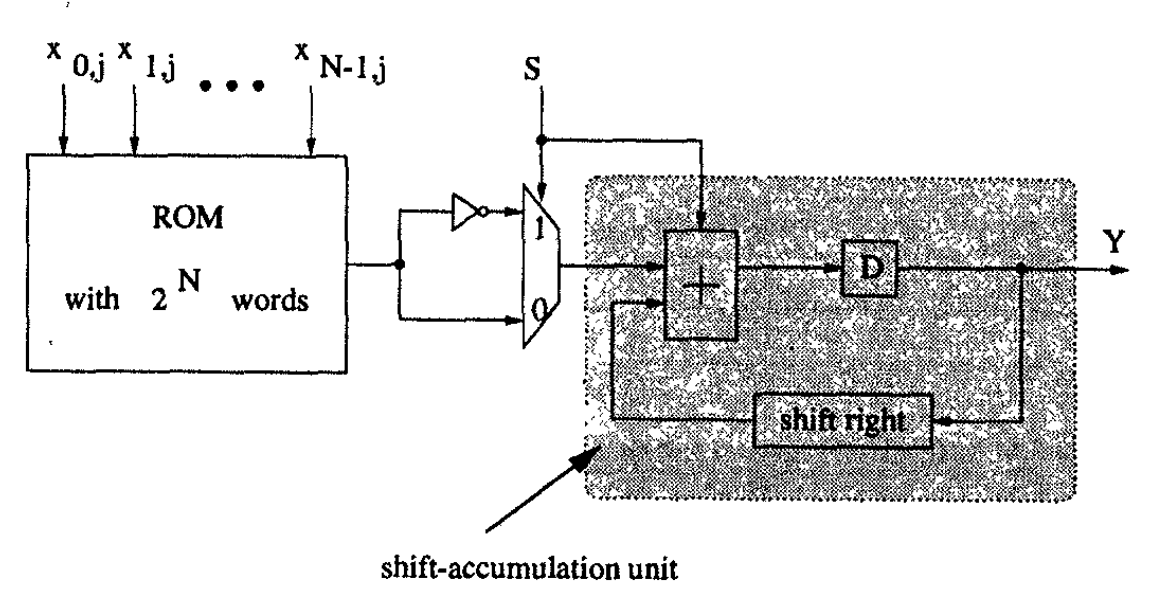
\includegraphics[scale=0.35]{images/da.png}
\end{figure}
Figure % figure number here
shows a typical architecture for computing inner product of two length-$N$ vectors using Distributed Arithmetic. The shift-accumulator is a bit-parallel carry-propagate adder that adds the ROM output to the previous adder output. The control signal $S$ is 1 when $j = W-1$ and 0 otherwise to invert the ROM output in order to calculate $C_{W-1}$. This inversion is achieved with the help of the MUX and the inverter. The result is accumulated in the adder after $W$ clock cycles($j=0$ to $j=W-1$).

\begin{center}
% \begin{tabular}{ |c|c|c|c|c| }
\begin{tabular}{ |>{\centering\arraybackslash}m{1cm}|>{\centering\arraybackslash}m{1cm}|>{\centering\arraybackslash}m{1cm}|>{\centering\arraybackslash}m{1cm}|>{\centering\arraybackslash}m{4cm}| }
\hline
$x_{0,j}$ & $x_{1,j}$ & $x_{2,j}$ & $x_{3,j}$ & ROM\\
\hline
0 & 0 & 0 & 0 & 0 \\
\hline
0 & 0 & 0 & 1 & $c_3$\\
\hline
0 & 0 & 1 & 0 & $c_2$\\
\hline
0 & 0 & 1 & 1 & $c_2+c_3$\\
\hline
0 & 1 & 0 & 0 & $c_1$\\
\hline
0 & 1 & 0 & 1 & $c_1+c_3$\\
\hline
0 & 1 & 1 & 0 & $c_1+c_2$\\
\hline
0 & 1 & 1 & 1 & $c_1+c_2+c_3$\\
\hline
1 & 0 & 0 & 0 & $c_0$ \\
\hline
1 & 0 & 0 & 1 & $c_0+c_3$\\
\hline
1 & 0 & 1 & 0 & $c_0+c_2$\\
\hline
1 & 0 & 1 & 1 & $c_0+c_2+c_3$\\
\hline
1 & 1 & 0 & 0 & $c_0+c_1$\\
\hline
1 & 1 & 0 & 1 & $c_0+c_1+c_3$\\
\hline
1 & 1 & 1 & 0 & $c_0+c_1+c_2$\\
\hline
1 & 1 & 1 & 1 & $c_0+c_1+c_2+c_3$\\
\hline
\end{tabular}
\end{center}




\section{ROM Decomposition}
\begin{figure}[h]
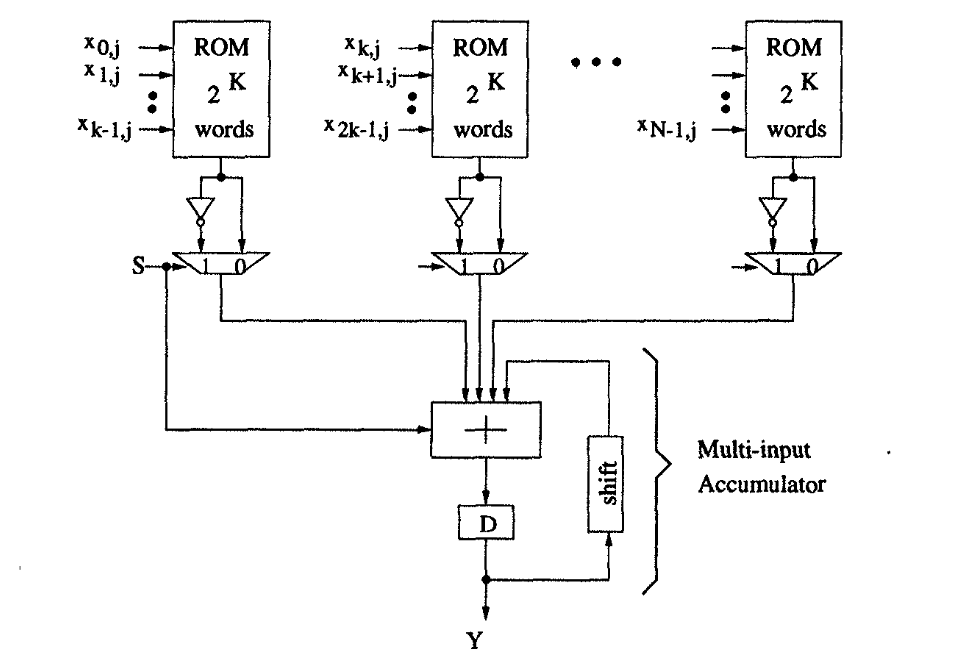
\includegraphics[scale=0.4]{images/da_decom.png}
\end{figure}
The ROM size of distributed arithmetic increases exponentially with the vector size $N$($2^N$) which along with the access time can bottleneck the speed of the whole system. The ROM size and access time can be improved by trading off the size with computational complexity of the accumulator.
The ROM size of the conventional DA and OBC based DA increases exponentially with the vector size $N$ ($2^N$ in conventional DA and $2^{N-1}$ in OBC based DA). When the ROM size is large, the ROM access time can limit the speed of the system. Hence, decreasing the ROM size is a very significant issue.

ROM decomposition provides a way to decrease the ROM size by trading off the ROM size with computational complexity. This can be achieved by dividing the $N$ address bits of the ROM into $N/K$ groups of $K$ bits effectively dividing or decomposing the ROM of size $2^N$ into $N/K$ ROMs of size $2^K$. This reduction in ROM size is at the cost of a multi-input accumulator to add the $N/K$ ROM outputs.
The total ROM size is now $(N/K)2^K$ which is a linear function of $N$ as opposed to an exponential increase.



\section{Offset Binary Coding}
Offset Binary Coding(OBC) based DA can reduce the ROM size from $2^N$ to $2^N-1$.
We write $x_i$ as
\begin{equation}\label{eqn:eq5}
\begin{split}
x_i &= \frac{1}{2}[x_i-(-x_i)]\\
    &= \frac{1}{2}[ -(x_{i, W-1}-\overline{x_{i, W-1}}) + \sum_{j=1}^{W-1}(x_{i, W-1-j} -\overline{x_{i, W-1-j}})2^{-j} - 2^{-(W-1)}]
\end{split}
\end{equation}
where $-x_i$ is
\begin{equation}
-x_i = -\overline{x_{i, W-1}} + \sum_{j=1}^{W-1}\overline{x_{i, W-1-j}}2^{-j} + 2^{-(W-1)}
\end{equation}
Define $d_{i,j}$ as
\begin{equation}\label{eqn:eq6}
d_{i,j} =
\begin{cases}
x_{i,j} - \overline{x_{i,j}},\ for \  j\neq W-1\\
-(x_{i, W-1} - \overline{x_{i, W-1}}),\ for\ j=W-1
\end{cases}
\end{equation}
Rewrite \eqref{eqn:eq5} using \eqref{eqn:eq6}
\begin{equation}\label{eqn:eq7}
x_i = \frac{1}{2}[\sum_{j=0}^{W-1}d_{i, W-1-j}2^{-j} - 2^{-(W-1)}]
\end{equation}
From \eqref{eqn:eq7} and \eqref{eqn:eq1}
\begin{equation}\label{eqn:eq8}
\begin{split}
Y &= \sum_{i=0}^{N-1}c_i[\frac{1}{2}(\sum_{j=0}^{W-1}d_{i, W-1-j}2^{-j} - 2^{-(W-1)})]\\
  &= \sum_{j=0}^{W-1}(\sum_{i=0}^{N-1}\frac{1}{2}c_id_{i,W-1-j})2^{-j} - (\sum_{i=0}^{N-1}\frac{1}{2}c_i)2^{-(W-1)}
\end{split}
\end{equation}
Define $D_j$
\begin{equation}
D_j = \sum_{i=0}^{N-1}\frac{1}{2}c_id_{i,W-1-j},\ for\ j=0\ to\ W-1
\end{equation}
and $D_{extra}$
\begin{equation}
D_{extra} = \sum_{i=0}^{N-1}\frac{1}{2}c_i
\end{equation}
Substituting $D_j$'s and $D_{extra}$ into \eqref{eqn:eq8}
\begin{equation}
Y = \sum_{j=0}^{W-1}D_{W-1-j}2^{-j} + D_{extra}2^{-(W-1)}
\end{equation}

\begin{center}
% \begin{tabular}{ |c|c|c|c|c| }
\begin{tabular}{ |>{\centering\arraybackslash}m{1cm}|>{\centering\arraybackslash}m{1cm}|>{\centering\arraybackslash}m{1cm}|>{\centering\arraybackslash}m{1cm}|>{\centering\arraybackslash}m{5cm}| }
\hline
$x_{0,j}$ & $x_{1,j}$ & $x_{2,j}$ & $x_{3,j}$ & ROM\\
\hline
0 & 0 & 0 & 0 & $-(c_0+c_1+c_2+c_3)/2$\\
\hline
0 & 0 & 0 & 1 & $-(c_0+c_1+c_2-c_3)/2$\\
\hline
0 & 0 & 1 & 0 & $-(c_0+c_1-c_2+c_3)/2$\\
\hline
0 & 0 & 1 & 1 & $-(c_0+c_1-c_2-c_3)/2$\\
\hline
0 & 1 & 0 & 0 & $-(c_0-c_1+c_2+c_3)/2$\\
\hline
0 & 1 & 0 & 1 & $-(c_0-c_1+c_2-c_3)/2$\\
\hline
0 & 1 & 1 & 0 & $-(c_0-c_1-c_2+c_3)/2$\\
\hline
0 & 1 & 1 & 1 & $-(c_0-c_1-c_2-c_3)/2$\\
\hline
\hline
\hline
1 & 0 & 0 & 0 & $(c_0-c_1-c_2-c_3)/2$\\
\hline
1 & 0 & 0 & 1 & $(c_0-c_1-c_2+c_3)/2$\\
\hline
1 & 0 & 1 & 0 & $(c_0-c_1+c_2-c_3)/2$\\
\hline
1 & 0 & 1 & 1 & $(c_0-c_1+c_2+c_3)/2$\\
\hline
1 & 1 & 0 & 0 & $(c_0+c_1-c_2-c_3)/2$\\
\hline
1 & 1 & 0 & 1 & $(c_0+c_1-c_2+c_3)/2$\\
\hline
1 & 1 & 1 & 0 & $(c_0+c_1+c_2-c_3)/2$\\
\hline
1 & 1 & 1 & 1 & $(c_0+c_1+c_2+c_3)/2$\\
\hline
\end{tabular}
\end{center}
The contents of the ROM have inverse symmetry as observed from the lookup table. This symmetry can be exploited to reduce the number of possible combinations by a factor of 2 reducing the ROM size by half.
\begin{figure}[h]
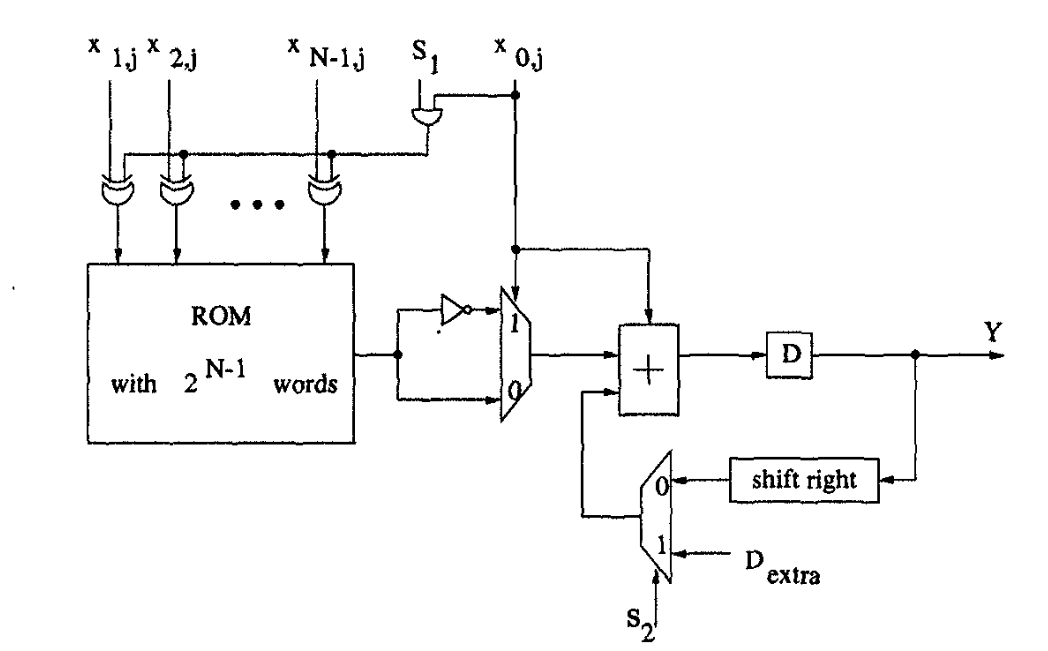
\includegraphics[scale=0.35]{images/da_obc.png}
\end{figure}

% figure number here
Figure shows a typical architecture for computing inner product of two length-$N$ vectors using OBC based DA. The architecture is mostly the same as conventional DA.

Control signal $S_2$ is 1 when $j=0$ and 0 otherwise providing the initial value $D_{extra}$ to the shift-accumulator. The XOR gates are used to select the correct address. The MUX after the ROM inverts the ROM output depending on the sign bit.


\section{Applying Distributed Arithmetic to LSTM}
% refer lstm equations
Refer to LSTM cell equations 
A simplified version can be written as $f(Wx+b)$ where $f$ is a non-linear activation function. The $Wx+b$ part can be optimized using DA. Write $W$ as
\begin{equation}
W = [w_0, w_1, w_2, w_3 ..., w_N-1]
\end{equation}
where $w_i$'s are column vectors of $W$ and x is a column vector.
So $Wx$ can be written as 
\begin{equation}
Wx = [w_0.x, w_1.x, w_2.x, w_3.x ..., w_N-1.x]^\top
\end{equation}

\chapter{Proposed Algorithm and Architecture}
\label{paaa}
\section{Profiling an LSTM}
Since the primary objective of our work is to develop an implementation of an LSTM on hardware with minimal power, compute and memory requirement, we will need to first identify what operations in the network's structure occupies the most compute power. The following methodology was adopted to profile the LSTM.\\
A 2 Layer LSTM with 128 hidden units each was implemented in $Tensorflow$, a computation graph library for deep neural networks and the $Profiler$ tool of the library was used to find the number of floating-point operations(FLOPs) each broad category of operation required. The results are represented graphically below.

\begin{figure}[h]
\caption{Profile of LSTM Network}
\centering
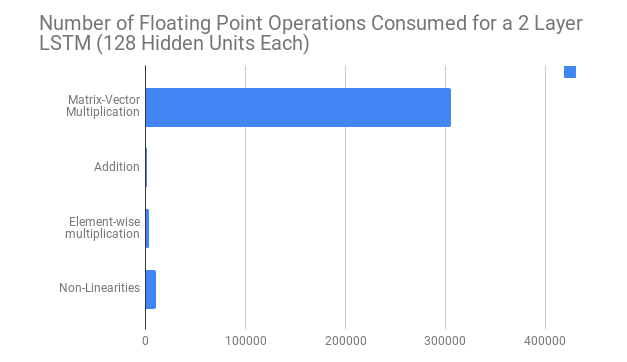
\includegraphics[width=0.8\textwidth]{profile}
\end{figure}

The following conclusions can be drawn from the above graph:
\begin{itemize}
    \item The most computationally expensive operation is the \textbf{matrix-vector multiplication}. Of the matrix and the vector, the vector or the input changes every time instant but the matrix is constant for a particular network regardless of the input. This needs to leveraged when optimizing the network
    \item The next most computationally expensive operation are the \textbf{non-linearities} $sigmoid$ and $tanh$.
    \item \textbf{Element-wise multiplication} and \textbf{addition} operations are insignificant in comparison with the other operations.
\end{itemize}

\section{Matrix-Vector Multiplication}
constant matrix and matmul is the most expensive operation. leads to DA being a possible option

As mentioned above, the matrix-vector multiplication operation is the one that needs to be tackled first. Since the weight matrices are constant for a particular network, distributed arithmetic can be seen as a possible solution to implement the multiplication operation. DA removes the need for a multiplier in the circuit. Therefore, below, DA and its various optimizations are elaborated and applied to task of matrix-vector multiplication. The memory requirement is then analysed and further avenues to reduce this are proposed.
\subsection{Distributed Arithmetic}
\subsubsection{Offset Binary Coding}
\subsubsection{ROM Decomposition}
\subsubsection{Applying DA to LSTMs}
tell the current memory requirement
\subsection{Network Compression}
\subsubsection{Pruning}
\subsubsection{Quantization}
\subsubsection{Low Displacement Rank Methods}
\subsubsection{Knowledge Distillation}
\subsubsection{Logic Based without DA}

-Pruning creates 90\% sparsity. Is it possible to exploit??? cite the sparse DA paper.
-Quantization - need to store less, but indexing is more problematic
-Knowledge Distillation has shown to reduce model size ~5x( read the paper)
-No memory, direct logic gates

\chapter{Future Work}
A majority of the work that has been done is to come up to speed with the current paradigms in compression of a network and also familiarising with the Digital Signal Processing techniques for optimizing VLSI implementations. The future work can be broadly classified into three phases:
\begin{enumerate}
\item \textbf{Finalising the architecture of the Network:} The first step is to finalize on the compressed model by experimenting with the various techniques described in Network Compression chapter. This involves trying pruning alone, pruning with quantization and also experimenting with knowledge distillation and sparse matrix decompositions of the weight matrices.
\item \textbf{Memory management and DA architecture:} In tandem with step 1, the final optimized structure of DA including ROM decomposition and OBC has to be constructed. Also, the different levels of memory i.e., deciding the on-board SRAM memory size and off-chip DRAM memory size and arrangement have to be decided.
\item \textbf{Non-linear activations:} The non-linear functions $sigmoid$ and $tanh$ introduces additional latency in the model. Linearizing these functions piecewise can lead to a speedup of the network.
\item \textbf{Pipelining:} This involves two distinct approaches. The first is to pipeline the tasks inside a single LSTM cell. The other avenue of pipelining is to treat the LSTM cell as a black box and pipeline the different the layers of the network.
\end{enumerate}           % Chapter 4: Analysis
            % Chapter 5: Simulation and Results
%\include{conclusion}         % Chapter 6: Finally the summary & conclusions
\end{spacing}

%=====================================================================
% APPENDIX
%  Appendices, if any, must precede the cited literatures.
%  Appendices shall be numbered in Roman Capitals (e.g. Appendix IV)

%% \appendix
%% \include{appendix_something}

%=====================================================================
% BIBLIOGRAPHY
%   This should follow the appendices, if any, otherwise summary and
%   conclusions chapter.
% Choose your bibliography style
% plain is the basic style, others include ieeetr, siam, asm, etc
%\bibliographystyle{plain}
% Add the bib file
%% \bibliography{bibfile}

\begin{thebibliography}{10}
\begin{small}

\bibitem{ref:FCC}
``Spectrum Policy Task Force Report,'' {\em Federal Commun.\ Commission,\ Tech.\ Rep.}, Nov.~2002.\\
 Available at http://hraunfoss.fcc.gov/edocs\_publish/attachmatch/DOC-228542A1.pdf

\bibitem{ref:haykin}
S. Haykin, ``Cognitive Radio: Brain Empowered Wireless Communications,'' {\em IEEE Journal on Selected Areas in Communication}, Vol.~23, No.~2, pp.~201-�220, Feb.~2005.

\end{small}
\end{thebibliography}
%=====================================================================
% PUBLICATIONS
%  publications if any may be listed after the literature cited.
%% \include{mypubs}

%=====================================================================


\end{document} 
